\documentclass{ctexart}
\usepackage{geometry}
\usepackage{fancyhdr}
\usepackage{graphicx}
\usepackage{booktabs}
\usepackage{amsmath}
\usepackage{multirow}
\usepackage{float}
\usepackage{tikz}
\usepackage{array}
\xeCJKsetup{CJKmath=true} 
\usepackage{zhnumber} % change section number to chinese
\renewcommand\thesection{\zhnum{section}}
\renewcommand \thesubsection {\arabic{subsection}}
\CTEXsetup[format={\Large\bfseries}]{section}

\geometry{
    a4paper,
    left=3.18cm,
    right=3.18cm,
    top=3.04cm,
    bottom=3.04cm
}

\pagestyle{fancy}
\fancyhf{}
\renewcommand{\headrulewidth}{0.7pt} % 设置页眉横线粗细
\fancyhead[L]{\kaishu\large 大学物理实验报告} % 在左侧设置页眉文字
\fancyhead[R]{\kaishu\large 哈尔滨工业大学(深圳) } % 在右侧设置页眉文字
\fancyfoot[R]{\thepage} % 将页数放在右下角


\setlength\headwidth{\textwidth}

\begin{document}

\noindent
\begin{center}
\textbf{
\begin{tabular}{p{2.4cm}p{2.4cm}p{4cm}p{4cm}}
    班级 \hrulefill & 学号 \hrulefill & 姓名 \hrulefill & 教师签字 \hrulefill \\
\end{tabular}
\begin{tabular}{p{6cm}p{3.6cm}p{3.6cm}}
    实验日期 \hrulefill & 预习成绩 \hrulefill & 总成绩 \hrulefill
\end{tabular}
{\noindent}	 \rule[-10pt]{\textwidth}{0.7pt}
}\end{center}

\begin{center}
    \Large \textbf{实验内容 \underline{分光计的调节及应用}}
\end{center}

\section{预习内容}

\subsection{分光计调节的主要步骤与要点;}
\subsection{如何调整望远镜光轴与分光计的中心轴垂直,何为“各半调节法(对半调节法)”?}
\subsection{衍射光栅测定光的波长工作原理是什么?}

\newpage
\section{数据记录}

\begin{table}[h]
    \renewcommand{\arraystretch}{1.3} % 表格行高倍数
    \centering
    \caption{用衍射光栅测定光的波长实验数据}
    \begin{tabular}{|c|c|m{1cm}<{\centering}|m{1cm}<{\centering}|m{1cm}<{\centering}|m{1cm}<{\centering}|c|}
    \hline
    \multirow{2}*{颜色} & \multirow{2}*{衍射级数$k$} & \multicolumn{2}{c|}{$+$} & \multicolumn{2}{c|}{$-$} & \multirow{2}*{标准波长 $(nm)$} \\
    \cline{3-6}
    & & $\theta_1$ & $\theta_2$ & $\theta_1'$ & $\theta_2'$ &\\
    \hline
    \multirow{3}*{绿} & 1 &  &  &  &  & \multirow{3}*{$546.1$} \\
    \cline{2-6}
    & 2 &  &  &  &  & \\
    \cline{2-6}
    & 3 &  &  &  &  & \\
    \hline
    \multirow{3}*{黄$1$} & 1 &  &  &  &  & \multirow{3}*{$577.0$} \\
    \cline{2-6}
    & 2 &  &  &  &  & \\
    \cline{2-6}
    & 3 &  &  &  &  & \\
    \hline
    \multirow{3}*{黄$2$} & 1 &  &  &  &  & \multirow{3}*{$579.1$} \\
    \cline{2-6}
    & 2 &  &  &  &  & \\
    \cline{2-6}
    & 3 &  &  &  &  & \\
    \hline
    \end{tabular}
\end{table}

\begin{table}[h]
    \renewcommand{\arraystretch}{1.3}
    \centering
    \caption{用衍射光栅测定光的波长实验数据}
    \begin{tabular}{|c|m{1cm}<{\centering}|m{1cm}<{\centering}|m{1cm}<{\centering}|m{1cm}<{\centering}|}
    \hline
    操作& $\theta_1$ & $\theta_2$ & $\theta_1'$ & $\theta_2'$ \\
    \hline
    测三棱镜顶角&&&&\\
    \hline
    测三棱镜最小偏向角&&&&\\
    \hline
    \end{tabular}
\end{table}

\begin{tikzpicture}[remember picture,overlay]
    \node[anchor=south east,inner sep=100pt] at (current page.south east) {
        \renewcommand{\arraystretch}{1.5} % 表格行高倍数
        \setlength{\tabcolsep}{18pt}    
    \begin{tabular}{|c|c|}
        \hline
        \LARGE  教师 & \LARGE  姓名 \\
        \hline
        \LARGE \kaishu 签字 &  \\
        \hline
        \end{tabular}
    };
\end{tikzpicture}

\newpage

\section{数据处理}

\subsection{分别计算相应三种颜色的光(绿光、黄光1、黄光2)在衍射级次$k=1、2、3$时波长的测量值$\lambda_k$,并计算波长平均值$\overline{\lambda}$,将$\overline{\lambda}$与汞灯波长的标准值相比较,计算测量的相对误差。要求写出完整的计算过程,包括所用公式和代入实验数据后的表达式。}

根据实验原理进行计算,可以得到:

$$ \psi_k = \left[(\theta_1'-\theta_1)+(\theta_2'-\theta_2)\right]/4 $$

带入实验数据,使用计算机循环计算得到下表:
\begin{table}[!h]
    \centering
    \begin{tabular}{c ccc}
        \toprule
        \textbf{颜色} & $\psi_1$ & $\psi_2$ & $\psi_3$ \\
        \midrule
        \textbf{绿光} & $9^\circ 25' 0"$ & $19^\circ 6' 45"$ & $29^\circ 25' 30"$\\
        \textbf{黄光1} & $9^\circ 58' 0"$ & $20^\circ 14' 15"$ & $31^\circ 16' 15"$\\
        \textbf{黄光2} & $10^\circ 1' 0"$ & $20^\circ 18' 45"$ & $31^\circ 22' 45"$\\
        \bottomrule
    \end{tabular}
\end{table}

然后我们使用数据计算波长,套入理论公式,循环计算得到下表:(其中$d=1/300mm$,保留三位小数)

$$ \lambda_k = \frac{d\sin\psi_k}{k} $$

\begin{table}[!h]
    \centering
    \begin{tabular}{c ccc}
        \toprule
        \textbf{颜色} & $\lambda_1$ & $\lambda_2$ & $\lambda_3$ \\
        \midrule
        \textbf{绿光} & $545.376$ & $545.707$ & $545.871$\\
        \textbf{黄光1} & $576.917$ & $576.521$ & $576.76$\\
        \textbf{黄光2} & $579.782$ & $578.567$ & $578.555$\\
        \bottomrule
    \end{tabular}
\end{table}

进而计算平均波长以及相对误差,得到计算结果如下:

$$ \overline{\lambda} = \frac{\lambda_1+\lambda_2+\lambda_3}{3} $$

$$ \varepsilon = \frac{\left|\overline{\lambda}-\lambda_{std}\right|}{\lambda_{std}} \times 100\% $$



\begin{table}[!h]
    \centering
    \begin{tabular}{c ccc}
        \toprule
        \textbf{颜色} & \textbf{绿光} & \textbf{黄光1} & \textbf{黄光2}\\
        \midrule
        $\lambda_{std}$ & $546.1$ & $577.0$ & $579.1$\\
        $\overline{\lambda}$ & $545.651$ & $576.733$ & $578.968$\\
        $\varepsilon$ & $0.082\% $ & $0.046\% $ & $0.023\% $\\
        \bottomrule
    \end{tabular}
\end{table}




\subsection{计算衍射光栅对黄光1和黄光2在衍射级次$k=1、2、3$时的角色散率$D_k$。}

角色散率即衍射角对波长的导数,由光栅方程推导得到:

$$ D_k = \frac{\mathrm{d}\theta}{\mathrm{d}\lambda} = \frac{k}{d\cos\psi_k} $$

带入实验数据,得到计算结果如下:

\begin{table}[!h]
    \centering
    \begin{tabular}{c ccc}
        \toprule
        \textbf{颜色} & \textbf{黄光1} & \textbf{黄光2} \\
        \midrule
        $D_1$ & 0.304597 & 0.304644 \\
        $D_2$ & 0.639477 & 0.639786 \\
        $D_3$ & 1.052972 & 1.054185 \\
        \bottomrule
    \end{tabular}
\end{table}

\subsection{计算三棱镜的顶角、绿光对应的最小偏向角,计算三棱镜材料对绿光的折射率。}

根据实验原理,同一游标的两次读数之差$ \left|\theta_1 - \theta_1'\right| $,$ \left|\theta_2 - \theta_2'\right| $的平均值即为载物台转过的角度$\varPhi $,于是:

$$ A = \pi - \frac{\left|\theta_1 - \theta_1'\right|+\left|\theta_2 - \theta_2'\right|}{2} $$

计算得到数值为$ A = 60^\circ 15' $

下一步计算三棱镜最小偏向角,根据实验原理,可以得到:

$$ \delta_{min} = \frac{\left|\theta_1 - \theta_1'\right|+\left|\theta_2 - \theta_2'\right|}{2} $$

计算结果为$ \delta_{min} = 128^\circ 37' $

最后计算三棱镜材料对绿光的折射率,易有:

$$ n = \frac{\sin\left(\frac{A+\delta_{min}}{2}\right)}{\sin\left(\frac{A}{2}\right)} = 1.64826 $$

\newpage

\section{讨论题}

\subsection{应用分光计进行测量之前,应调节到何种状态?}

应当调整使得望远镜对焦到无穷远,然后调整望远镜光轴与分光计载物台的中心轴垂直,即使得两者的光轴重合;其次要使得平行光管与望远镜光轴同轴,然后需要调整调整狭缝宽度,以获取适当的光强和分辨率。

\subsection{按游标原理,读出下图中的角度数。}

\begin{figure}[!ht]
    \centering
    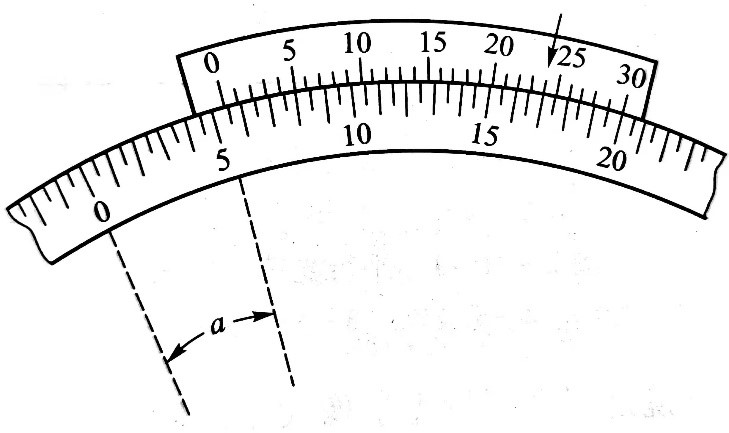
\includegraphics[width=0.6\textwidth]{./1.jpg}
\end{figure}

显然有读数为 $ 5^\circ 24' $

\end{document}